

%🍁% \chapter{Classes and functions}
\chapter{类和函数}
\label{time}

%🍁% Now that we know how to create new types, the next
%🍁% step is to write functions that take programmer-defined objects
%🍁% as parameters and return them as results.  In this chapter I
%🍁% also present ``functional programming style'' and two new
%🍁% program development plans.

现在我们已经知道如何去定义一个新的类型,下一步就是编写以自定义对象为参数的函数,并返回自定义对象作为结果。在本章中,我还将介绍“函数式编程风格”和两种新的编程开发方案。

%🍁% Code examples from this chapter are available from
%🍁% \url{http://thinkpython2.com/code/Time1.py}.
%🍁% Solutions to the exercises are at
%🍁% \url{http://thinkpython2.com/code/Time1_soln.py}.

本章的代码示例可以从 \href{http://thinkpython2.com/code/Time1.py}{这里} 下载。  练习的答案可以从 \href{http://thinkpython2.com/code/Time1_soln.py}{这里} 下载。

%🍁% \section{Time}
\section{时间}
\label{isafter}

%🍁% As another example of a programmer-defined type, we'll define a class
%🍁% called {\tt Time} that records the time of day.  The class definition
%🍁% looks like this: \index{programmer-defined type}

再举一例程序员自定义的类型,我们定义一个叫 \li{Time} 的类,用于记录时间。
这个类将如下定义:
\index{type!programmer-defined} \index{Time class} \index{class!Time}

\begin{lstlisting}
class Time:
    """Represents the time of day.

    attributes: hour, minute, second
    """
\end{lstlisting}

%
%🍁% We can create a new {\tt Time} object and assign
%🍁% attributes for hours, minutes, and seconds:

我们可以创建一个新的 \li{Time} 类对象,并且给它的属性 \li{hour} ,
\li{minutes} 和 \li{seconds} 赋值:

\begin{lstlisting}
time = Time()
time.hour = 11
time.minute = 59
time.second = 30
\end{lstlisting}

%
%🍁% The state diagram for the {\tt Time} object looks like Figure~\ref{fig.time}.

\li{Time} 对象的状态图类似于 图~\ref{fig.time}。

\index{state diagram}  \index{diagram!state}
\index{object diagram}  \index{diagram!object}

%🍁% As an exercise, write a function called \verb"print_time" that takes a
%🍁% Time object and prints it in the form {\tt hour:minute:second}.
%🍁% Hint: the format sequence \verb"'%.2d'" prints an integer using
%🍁% at least two digits, including a leading zero if necessary.

我们做个练习,编写一个叫做 \li{print_time} 的函数,
接收一个 \li{Time} 对象并用 \li{时:分:秒} 的格式打印它。
提示:格式化序列 \li{%.2d} 可以至少两位数的形式打印一个整数,如果不足则在前面补0。

%🍁% Write a boolean function called \verb"is_after" that
%🍁% takes two Time objects, {\tt t1} and {\tt t2}, and
%🍁% returns {\tt True} if {\tt t1} follows {\tt t2} chronologically and
%🍁% {\tt False} otherwise.  Challenge: don't use an {\tt if} statement.

编写一个叫做 \li{is_after} 的布尔函数,接收两个 \li{Time}  对象, \li{t1}  和 \li{t2} ,若 \li{t1} 的时间在 \li{t2} 之后,
则返回 \li{True} ,否则返回 \li{False} 。 挑战:不要使用 \li{if} 语句。

\begin{figure}
\centerline
{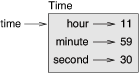
\includegraphics[scale=0.8]{../source/figs/time.pdf}}
%🍁%\caption{Object diagram.}
\caption{对象图。}
\label{fig.time}
\end{figure}

%🍁% \section{Pure functions}
\section{纯函数}
\index{prototype and patch}  \index{development plan!prototype and patch}

%🍁% In the next few sections, we'll write two functions that add time
%🍁% values.  They demonstrate two kinds of functions: pure functions and
%🍁% modifiers.  They also demonstrate a development plan I'll call {\bf
%🍁%   prototype and patch}, which is a way of tackling a complex problem
%🍁% by starting with a simple prototype and incrementally dealing with the
%🍁% complications.
%🍁%
%🍁% Here is a simple prototype of \verb"add_time":

下面几节中,我们将编写两个用来增加时间值的函数。
它们展示了两种不同的函数: {\em 纯函数} (pure functions) 和
{\em 修改器} (modifiers)。
它们也展示了我所称的 {\em 原型和补丁} (prototype and patch) 的开发方案。
这是一种处理复杂问题的方法, 从简单的原型开始, 逐步解决复杂情况。

下面是一个简单的 \li{add_time} 原型:

\begin{lstlisting}
def add_time(t1, t2):
    sum = Time()
    sum.hour = t1.hour + t2.hour
    sum.minute = t1.minute + t2.minute
    sum.second = t1.second + t2.second
    return sum
\end{lstlisting}

%🍁% %
%🍁% The function creates a new {\tt Time} object, initializes its
%🍁% attributes, and returns a reference to the new object.  This is called
%🍁% a {\bf pure function} because it does not modify any of the objects
%🍁% passed to it as arguments and it has no effect,
%🍁% like displaying a value or getting user input,
%🍁% other than returning a value.

这个函数创建了一个新的 \li{Time}
对象,初始化了对象的属性,并返回了这个对象的引用。
我们把这个函数称为 {\em 纯函数} (pure function),
因为它除了返回一个值以外, 并不修改作为参数传入的任何对象,
也没有产生如显示一个值或者获取用户输入的影响。

\index{pure function}  \index{function type!pure}

%🍁% To test this function, I'll create two Time objects: {\tt start}
%🍁% contains the start time of a movie, like {\em Monty Python and the
%🍁% Holy Grail}, and {\tt duration} contains the run time of the movie,
%🍁% which is one hour 35 minutes.

\index{Monty Python and the Holy Grail}

%🍁% \verb"add_time" figures out when the movie will be done.

为了测试这个函数,我将创建两个 \li{Time} 对象: \li{start} 用于存放一个电影
(如 Monty Python and the Holy Grail)的开始时间, \li{duration} 用于存放电影的放映时长,这里时长定为 1 小时 35 分钟。

\li{add_time} 将计算电影何时结束。


\begin{lstlisting}
>>> start = Time()
>>> start.hour = 9
>>> start.minute = 45
>>> start.second =  0

>>> duration = Time()
>>> duration.hour = 1
>>> duration.minute = 35
>>> duration.second = 0

>>> done = add_time(start, duration)
>>> print_time(done)
10:80:00
\end{lstlisting}

%🍁% %
%🍁% The result, {\tt 10:80:00} might not be what you were hoping
%🍁% for.  The problem is that this function does not deal with cases where the
%🍁% number of seconds or minutes adds up to more than sixty.  When that
%🍁% happens, we have to ``carry'' the extra seconds into the minute column
%🍁% or the extra minutes into the hour column.
\index{carrying, addition with}

%🍁% Here's an improved version:

这个结果 \li{10:80:00} 可能不是你所希望得到的。
问题在于这个函数并没有处理好秒数和分钟数相加超过60的情况。
当发生这种情况时,我们要把多余的秒数放进分钟栏,或者把多余的分钟加进小时栏。

下面是一个改进的版本:

\begin{lstlisting}
def add_time(t1, t2):
    sum = Time()
    sum.hour = t1.hour + t2.hour
    sum.minute = t1.minute + t2.minute
    sum.second = t1.second + t2.second

    if sum.second >= 60:
        sum.second -= 60
        sum.minute += 1

    if sum.minute >= 60:
        sum.minute -= 60
        sum.hour += 1

    return sum
\end{lstlisting}

%🍁% %
%🍁% Although this function is correct, it is starting to get big.
%🍁% We will see a shorter alternative later.

这个函数虽然正确,但是它开始变得臃肿。我们会在后面看到一个较短的版本。

%🍁% \section{Modifiers}
\section{修改器}

\label{increment}
\index{modifier}  \index{function type!modifier}

%🍁% Sometimes it is useful for a function to modify the objects it gets as
%🍁% parameters.  In that case, the changes are visible to the caller.
%🍁% Functions that work this way are called {\bf modifiers}.、

有时候用函数修改作为参数传入的对象是很有用的。在这种情况下,这种改变对
调用者来说是可见的。这种方式工作的函数称为 {\em 修改器} (modifiers)。

\index{increment}

%🍁% {\tt increment}, which adds a given number of seconds to a {\tt Time}
%🍁% object, can be written naturally as a
%🍁% modifier.  Here is a rough draft:

函数 \li{increment} 给一个 \li{Time} 对象增加指定的秒数,
可以很自然地用修改器来编写。  下面是一个原型:

\begin{lstlisting}
def increment(time, seconds):
    time.second += seconds

    if time.second >= 60:
        time.second -= 60
        time.minute += 1

    if time.minute >= 60:
        time.minute -= 60
        time.hour += 1
\end{lstlisting}

%🍁% %
%🍁% The first line performs the basic operation; the remainder deals
%🍁% with the special cases we saw before.

第一行进行基础操作;其余部分的处理则是我们之前看到的特殊情况。

\index{special case}

%🍁% Is this function correct?  What happens if {\tt seconds}
%🍁% is much greater than sixty?

这个函数正确吗? 如果 \li{seconds} 比 60 大很多会发生什么?

%🍁% In that case, it is not enough to carry once; we have to keep doing it
%🍁% until {\tt time.second} is less than sixty.  One solution is to
%🍁% replace the {\tt if} statements with {\tt while} statements.  That
%🍁% would make the function correct, but not very efficient.  As an
%🍁% exercise, write a correct version of {\tt increment} that doesn't
%🍁% contain any loops.

在那种情况下,只进位一次是不够的;我们要重复执行直到 \li{seconds} 小于 60。
一种方法是用 \li{while} 语句代替 \li{if} 语句。
这样能够让函数正确,但是并不是很高效。

%🍁% Anything that can be done with modifiers can also be done with pure
%🍁% functions.  In fact, some programming languages only allow pure
%🍁% functions.  There is some evidence that programs that use pure
%🍁% functions are faster to develop and less error-prone than programs
%🍁% that use modifiers.  But modifiers are convenient at times,
%🍁% and functional programs tend to be less efficient.

任何能够用修改器实现的函数同样能够用纯函数实现。
事实上,一些编程语言只允许用纯函数。
一些证据表明用纯函数实现的程序比用修改器实现的函数开发更快、更不易出错。
但是有时候修改器是很方便的,而函数式程序效率反而不高。

%🍁% In general, I recommend that you write pure functions whenever it is
%🍁% reasonable and resort to modifiers only if there is a compelling
%🍁% advantage.  This approach might be called a {\bf functional
%🍁% programming style}.

通常来说,我推荐只要是合理的情况下,都使用纯函数方式编写,
只在有完全令人信服的原因下采用修改器。
这种方法可以称为 {\em 函数式编程风格} (functional programming style)。

\index{functional programming style}

%🍁% As an exercise, write a ``pure'' version of {\tt increment} that
%🍁% creates and returns a new Time object rather than modifying the
%🍁% parameter.

我们做个练习,编写一个纯函数版本的 \li{increment}  ,
创建并返回一个 \li{Time} 对象,而不是修改参数。


%🍁% \section{Prototyping versus planning}
\section{原型 {\em v.s.} 方案}

\label{prototype}
\index{prototype and patch}  \index{development plan!prototype and patch}
\index{planned development}  \index{development plan!designed}

%🍁% The development plan I am demonstrating is called ``prototype and
%🍁% patch''.  For each function, I wrote a prototype that performed the
%🍁% basic calculation and then tested it, patching errors along the
%🍁% way.

我刚才展示的开发方案叫做 {\em 原型和补丁} (protptype and patch) 。
针对每个函数,我编写了一个可以进行基本运算的原型并对其测试,逐步修正错误。

%🍁% This approach can be effective, especially if you don't yet have a
%🍁% deep understanding of the problem.  But incremental corrections can
%🍁% generate code that is unnecessarily complicated---since it deals with
%🍁% many special cases---and unreliable---since it is hard to know if you
%🍁% have found all the errors.

这种方法在你对问题没有深入理解时特别有效。但增量修正可能导致代码过度复杂,
因为需要处理许多特殊情况。也并不可靠,因为很难知道你是否已经找到了所有的错误。

%🍁% An alternative is {\bf designed development}, in which high-level
%🍁% insight into the problem can make the programming much easier.  In
%🍁% this case, the insight is that a Time object is really a three-digit
%🍁% number in base 60 (see \url{http://en.wikipedia.org/wiki/Sexagesimal}.)!  The
%🍁% {\tt second} attribute is the ``ones column'', the {\tt minute}
%🍁% attribute is the ``sixties column'', and the {\tt hour} attribute is
%🍁% the ``thirty-six hundreds column''.
\index{sexagesimal}

另一种方法叫做 {\em 设计开发} (designed development)。
对问题有高层次的理解能够使开发变得更容易。
这给我们的启示是,\li{Time} 对象本质上是一个基于六十进制的三位数\footnote{参考 \href{http://en.wikipedia.org/wiki/Sexagesimal}{维基百科} 。}!
属性 \li{second} 是``个位'',属性 \li{minute} 是 ``六十位'',属性 \li{hour} 是 ``360位数''。

%🍁% When we wrote \verb"add_time" and {\tt increment}, we were effectively
%🍁% doing addition in base 60, which is why we had to carry from one
%🍁% column to the next.
\index{carrying, addition with}
\index{维基百科}

当我们编写 \li{add_time} 和 \li{increment} 时,其实是在基于六十进制累加,
所以我们需要把一位进位到下一位。

%🍁% This observation suggests another approach to the whole problem---we
%🍁% can convert Time objects to integers and take advantage of the fact
%🍁% that the computer knows how to do integer arithmetic.

这个观察意味着我们可以用另一种方法去解决整个问题——我们可以把
\li{Time} 对象转换为整数,并利用计算机知道如何进行整数运算的这个事实。

%🍁% Here is a function that converts Times to integers:

下面是一个把 \li{Time} 对象转成整数的函数:

\begin{lstlisting}
def time_to_int(time):
    minutes = time.hour * 60 + time.minute
    seconds = minutes * 60 + time.second
    return seconds
\end{lstlisting}

%
%🍁% And here is a function that converts an integer to a Time
%🍁% (recall that {\tt divmod} divides the first argument by the second
%🍁% and returns the quotient and remainder as a tuple).
\index{divmod}

下面则是一个把整数转换为 \li{Time} 对象(回忆一下 \li{divmod} 是用第一个参数除以第二个参数并以元组的形式返回商和余数)。

\begin{lstlisting}
def int_to_time(seconds):
    time = Time()
    minutes, time.second = divmod(seconds, 60)
    time.hour, time.minute = divmod(minutes, 60)
    return time
\end{lstlisting}

%
%🍁% You might have to think a bit, and run some tests, to convince
%🍁% yourself that these functions are correct.  One way to test them is to
%🍁% check that \verb"time_to_int(int_to_time(x)) == x" for many values of
%🍁% {\tt x}.  This is an example of a consistency check.
\index{consistency check}

你可能需要思考一下,并运行一些测试,以此来说服自己这些函数是正确的。
一种测试方法是对很多的 \li{x} 检查 \li{time_to_int(int_to_time(x)) == x}
是否正确。  这是一致性检查的例子。

%🍁% Once you are convinced they are correct, you can use them to
%🍁% rewrite \verb"add_time":

一旦你确信它们是正确的,你就能使用它们重写 \li{add_time} :

\begin{lstlisting}
def add_time(t1, t2):
    seconds = time_to_int(t1) + time_to_int(t2)
    return int_to_time(seconds)
\end{lstlisting}

%
%🍁% This version is shorter than the original, and easier to verify.  As
%🍁% an exercise, rewrite {\tt increment} using \verb"time_to_int" and
%🍁% \verb"int_to_time".

这个版本比先前的要更短,更容易校验。
我们再做个练习,使用 \li{time_to_int} 和 \li{int_to_time}
重写 \li{increment} 函数。

%🍁% In some ways, converting from base 60 to base 10 and back is harder
%🍁% than just dealing with times.  Base conversion is more abstract; our
%🍁% intuition for dealing with time values is better.

从某个方面来说,六十进制和十进制相互转换比处理时间更难些。 进制转换更加抽象;
我们解决时间值的想法是更好的。

%🍁% But if we have the insight to treat times as base 60 numbers and make
%🍁% the investment of writing the conversion functions (\verb"time_to_int"
%🍁% and \verb"int_to_time"), we get a program that is shorter, easier to
%🍁% read and debug, and more reliable.

但如果我们意识到把时间当作六十进制,并预先做好编写转换函数 (\li{time_to_int}
和 \li{int_to_time}) 的准备,我们就能获得一个更短、更易读、更可靠的程序。

%🍁% It is also easier to add features later.  For example, imagine
%🍁% subtracting two Times to find the duration between them.  The
%🍁% naive approach would be to implement subtraction with borrowing.
%🍁% Using the conversion functions would be easier and more likely to be
%🍁% correct.

这让我们日后更加容易添加其它功能。 例如,试想将两个 \li{Time}
对象相减来获得它们之间的时间间隔。
最简单的方法是使用借位来实现减法。 使用转换函数则更容易,也更容易正确。

\index{subtraction with borrowing}  \index{borrowing, subtraction with}
\index{generalization}

%🍁% Ironically, sometimes making a problem harder (or more general) makes it
%🍁% easier (because there are fewer special cases and fewer opportunities
%🍁% for error).

讽刺的是,有时候把一个问题变得更难(或更加普遍)反而能让它更加简单
(因为会有更少的特殊情况和更少出错的机会)。

%🍁% \section{Debugging}
\section{调试}
\index{debugging}

%🍁% A Time object is well-formed if the values of {\tt minute} and {\tt
%🍁% second} are between 0 and 60 (including 0 but not 60) and if
%🍁% {\tt hour} is positive.  {\tt hour} and {\tt minute} should be
%🍁% integral values, but we might allow {\tt second} to have a
%🍁% fraction part.
\index{invariant}

如果 \li{minute} 和 \li{second} 的值介于 0 和 60 之间
(包括 0 但不包括 60 ),并且 \li{hour} 是正值, 那么这个 \li{Time}
对象就是合法的。 \li{hour} 和 \li{minute} 应该是整数值,
但我们可能也允许  \li{second} 有小数部分。

%🍁% Requirements like these are called {\bf invariants} because
%🍁% they should always be true.  To put it a different way, if they
%🍁% are not true, something has gone wrong.

这样的要求称为 {\em 不变式} (invariants)。 因为它们应当总是为真。
换句话说,如果它们不为真,肯定是某些地方出错了。

%🍁% Writing code to check invariants can help detect errors
%🍁% and find their causes.  For example, you might have a function
%🍁% like \verb"valid_time" that takes a Time object and returns
%🍁% {\tt False} if it violates an invariant:

编写代码来检查不变式能够帮助检测错误并找到出错的原因。
例如,你可能会写一个 \li{valid_time} 这样的函数,
接受一个 \li{Time} 对象,并在违反不变式的条件下返回 \li{False} :

\begin{lstlisting}
def valid_time(time):
    if time.hour < 0 or time.minute < 0 or time.second < 0:
        return False
    if time.minute >= 60 or time.second >= 60:
        return False
    return True
\end{lstlisting}

%
%🍁% At the beginning of each function you could check the
%🍁% arguments to make sure they are valid:

在每个函数的开头,你可以检查参数,确认它们是否合法:

\index{raise statement}  \index{statement!raise}

\begin{lstlisting}
def add_time(t1, t2):
    if not valid_time(t1) or not valid_time(t2):
        raise ValueError('invalid Time object in add_time')
    seconds = time_to_int(t1) + time_to_int(t2)
    return int_to_time(seconds)
\end{lstlisting}

%
%🍁% Or you could use an {\bf assert statement}, which checks a given invariant
%🍁% and raises an exception if it fails:
\index{assert statement}  \index{statement!assert}

或者你可以使用 **assert语句**,检查一个给定的不变式并在失败的情况下抛出异常:

\begin{lstlisting}
def add_time(t1, t2):
    assert valid_time(t1) and valid_time(t2)
    seconds = time_to_int(t1) + time_to_int(t2)
    return int_to_time(seconds)
\end{lstlisting}

%
%🍁% {\tt assert} statements are useful because they distinguish
%🍁% code that deals with normal conditions from code
%🍁% that checks for errors.

\li{assert} 语句非常有用,因为它们区分了处理普通条件的代码和检查错误的代码。

%🍁% \section{Glossary}
\section{术语表}

%🍁% \begin{description}
%🍁%
%🍁% \item[prototype and patch:] A development plan that involves
%🍁% writing a rough draft of a program, testing, and correcting errors as
%🍁% they are found.
%🍁% \index{prototype and patch}
%🍁%
%🍁% \item[designed development:] A development plan that involves
%🍁% high-level insight into the problem and more planning than incremental
%🍁% development or prototype development.
%🍁% \index{designed development}
%🍁%
%🍁% \item[pure function:] A function that does not modify any of the objects it
%🍁% receives as arguments.  Most pure functions are fruitful.
%🍁% \index{pure function}
%🍁%
%🍁% \item[modifier:] A function that changes one or more of the objects it
%🍁%   receives as arguments.  Most modifiers are void; that is, they
%🍁%   return {\tt None}.  \index{modifier}
%🍁%
%🍁% \item[functional programming style:] A style of program design in which the
%🍁% majority of functions are pure.
%🍁% \index{functional programming style}
%🍁%
%🍁% \item[invariant:] A condition that should always be true during the
%🍁% execution of a program.
%🍁% \index{invariant}
%🍁%
%🍁% \item[assert statement:] A statement that check a condition and raises
%🍁% an exception if it fails.
%🍁% \index{assert statement}
%🍁% \index{statement!assert}
%🍁%
%🍁% \end{description}

\begin{description}

\item[原型和补丁 (prototype and patch):]
一种开发方案,编写一个程序的初稿,测试,发现错误时修正它们。
\index{prototype and patch}

\item[设计开发 (designed development):]
一种开发方案,需要对问题有更高层次的理解,比增量开发或原型开发更有计划性。
\index{designed development}

\item[纯函数 (pure function):] 一种不修改任何作为参数传入的对象的函数。大部分纯函数是有返回值的(fruitful)。
\index{pure function}

\item[修改器 (modifier):]
一种修改一个或多个作为参数传入的对象的函数。
大部分修改器没有返回值;即返回 \li{None}
\index{modifier}

\item[函数式编程风格 (functional programming style):]
一种程序设计风格,大部分函数为纯函数。
\index{functional programming style}

\item[不变式 (invariant):]
在程序执行过程中总是为真的条件。
\index{invariant}

\item[(assert statement):]
一种检查条件是否满足并在失败的情况下抛出异常的语句。
\index{assert statement}  \index{statement!assert}

\end{description}

%🍁% \section{Exercises}
\section{练习}
%🍁% Code examples from this chapter are available from
%🍁% \url{http://thinkpython2.com/code/Time1.py}; solutions to the
%🍁% exercises are available from \url{http://thinkpython2.com/code/Time1_soln.py}.

本章的代码示例可以在 \href{http://thinkpython2.com/code/Time1.py}{此处}下载;
练习的答案可以在 \href{http://thinkpython2.com/code/Time1_soln.py}{此处}下载。

\begin{exercise}

%🍁% Write a function called \verb"mul_time" that takes a Time object
%🍁% and a number and returns a new Time object that contains
%🍁% the product of the original Time and the number.
%🍁%
%🍁% Then use \verb"mul_time" to write a function that takes a Time
%🍁% object that represents the finishing time in a race, and a number
%🍁% that represents the distance, and returns a Time object that represents
%🍁% the average pace (time per mile).
%🍁% \index{running pace}

编写一个叫做 {\em \li{mul_time}} 的函数,接收一个 {\em \li{Time}} 对象和一个数,并返回一个新的 {\em \li{Time}} 对象,包含原始时间和数的乘积。

然后使用 {\em \li{mul_time}} 编写一个函数,接受一个表示比赛完赛时间的 {\em \li{Time}} 对象以及一个表示距离的数字,并返回一个用于表示平均配速(每英里所需时间)的 {\em \li{Time}} 对象。

\index{running pace}

\end{exercise}


\begin{exercise}
\index{datetime module}  \index{module!datetime}

%🍁% The {\tt datetime} module provides {\tt time} objects
%🍁% that are similar to the Time objects in this chapter, but
%🍁% they provide a rich set of methods and operators.  Read the
%🍁% documentation at \url{http://docs.python.org/3/library/datetime.html}.
%🍁%
%🍁% \begin{enumerate}
%🍁%
%🍁% \item Use the {\tt datetime} module to write a program that gets the
%🍁%   current date and prints the day of the week.
%🍁%
%🍁% \item Write a program that takes a birthday as input and prints the
%🍁%   user's age and the number of days, hours, minutes and seconds until
%🍁%   their next birthday.
%🍁% \index{birthday}
%🍁%
%🍁% \item For two people born on different days, there is a day when one
%🍁%   is twice as old as the other.  That's their Double Day.  Write a
%🍁%   program that takes two birthdays and computes their Double Day.
%🍁%
%🍁% \item For a little more challenge, write the more general version that
%🍁%   computes the day when one person is $n$ times older than the other.
%🍁% \index{Double Day}
%🍁%
%🍁% \end{enumerate}
%🍁%
%🍁% Solution: \url{http://thinkpython2.com/code/double.py}


{\em \li{datetime}} 模块提供的 {\em \li{time}} 对象,
和本章的 {\em \li{Time}} 对象类似, 但前者提供了更丰富的方法和操作符。
参考阅读 \href{http://docs.python.org/3/library/datetime.html}{相关文档}。

\begin{enumerate}

\item 使用 {\em \li{datetime}} 模块来编写一个程序,获取当前日期并打印当天是周几。

\item 编写一个程序,接受一个生日作为输入,并打印用户的年龄以及距离下个生日所需要的天数、小时数、分钟数和秒数。

\item 对于两个不在同一天出生的人来说,总有一天,一个人的出生天数是另一个人的两倍。
   我们把这一天称为 ``双倍日''。  编写一个程序,接受两个不同的出生日期,并计算他们的 ``双倍日''。

\item 再增加点挑战,编写一个更通用的版本,用于计算一个人出生天数是另一个人 $n$ 倍的日子。

\end{enumerate}

\href{http://thinkpython2.com/code/double.py}{参考答案}

\end{exercise}